\documentclass[10pt,onecolumn,a4paper]{article}
\usepackage{epsfig,graphicx,subfigure,amsthm,amsmath}
\usepackage{color,xcolor}     
\usepackage{xepersian}
\settextfont[Scale=1.2]{B NAZANIN_YASDL.COM.TTF}
\setlatintextfont[Scale=1]{Times New Roman}

\linespread{1.5}




\begin{document}


% \title{گزارش نهایی پروژه یادگیری ماشین} 

% \author{اعضای گروه:\\
% محمدصادق صادقی\\
% حسین خلیلی \\
% }

% \date{\today}

% \maketitle

\begin{titlepage}
    \centering
    \vfill
    \begin{center}
    
\includegraphics[width=14cm]{title.jpg} % also works with logo.pdf
    \end{center}
     \vfill
    {\bfseries\Large
        گزارش نهایی پروژه یادگیری ماشین\\
        \vskip2cm
        اعضای گروه :\\
     
        حامد غلامی \\     
        محمد صادق صادقی \\
        امیرحسین محمدی  \\
        حسین خلیلی\\
        \vskip 1cm
        دی‌ماه 1400 \\
        
    }    
    \vfill
   
    \vfill
    \vfill
\end{titlepage}


\tableofcontents
\pagebreak

\section{مقدمه}

در این پروژه هدف ما بررسی الگوریتم‌های طبقه‌بندی و خوشه‌بندی برای 5 دسته از اهنگ‌های لری، کردی، گیلکی، بندری و ترکی می‌باشد. به این منظور ما در گام اول، نحوه استخراج ویژگی‌ها و پیش‌پردازش داده‌های استخراج شده  را به طور کامل توضیح می‌دهیم و در مورد هر دسته‌ از ویژگی‌ها به طور خلاصه اطلاعاتی را بیان می‌کنیم. در بخش بعدی، سه الگوریتم طبقه‌بندی پرسپترون چندلایه، \lr{XGBoost}  و \lr{SVM} را بر روی داده‌های بدست آمده از گام قبلی اجرا کرده و نتایج بدست آمده را مورد تحلیل و بررسی قرار می‌دهیم. در این گام نتایج بدست آمده نشان دهنده عملکرد مناسب مدل‌های پیاده‌سازی شده می‌باشد، در گام آخر نیز دو الگوریتم خوشه‌بندی \lr{Kmeans} و \lr{Agglomerative}  به منظور خوشه‌بندی مجموعه داده‌ها استفاده می‌شود و نتایج بدست آمده مورد تحلیل و بررسی قرار می‌گیرد.

\pagebreak
\section{استخراج ویژگی‌ها و پیش‌پردازش داده‌ها}


برای ساختن طیقه بند ، نیاز به ویژگی های متفاوت از آهنگ های داده شده داریم. حال برای اینکه بتوانیم این ویژگی ها را استخراج کنیم یعضا نیاز است که به حوزه فرکانس موسیقی ها علاوه بر حوزه زمان موسیقی ها توجه کنیم ( و در مواردی هر دوی آن ها). به طور خلاصه ویژگی ها را میتوان به دسته های زیر تقسیم کرد: \\
\subsection{ویژگی‌های حوزه زمان}
نرخ عبور از صفر\lr{ (Zero Crossing Rate)}  ،میزان جذر میانگین مربعات انرژی \lr{RMSE}،انرژی  کوتاه مدت \lr{(STE)} ،  و آنتروپی شانون \\


\begin{figure}[h!]
        \centering
        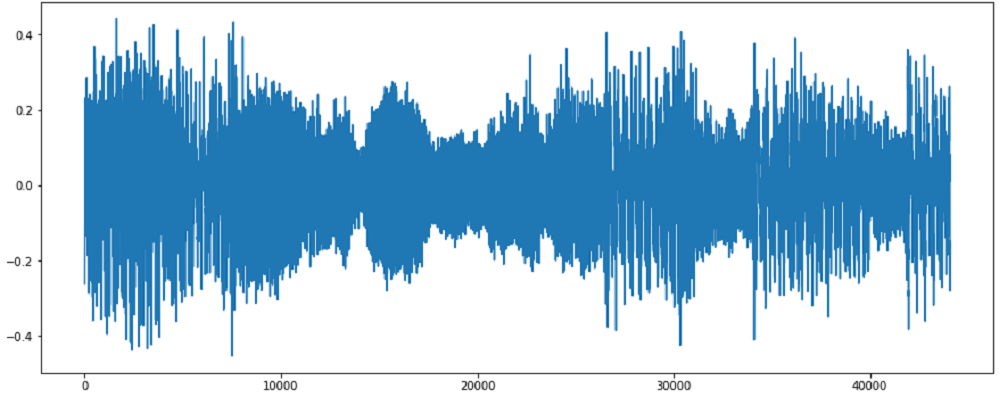
\includegraphics[scale=0.5]{1.png}
        \caption{\lr{Audio Signal in Time Domain(in one second) as we can see there can not be much be understood from raw  time domain.}  }  
    \end{figure}


\subsection{ویژگی‌های حوزه کپسترال}

 ضرایب کپسترال مبتنی بر فرکانس مل
\lr{ (Mel Frequency Cepstrul Coefiecients MFCC)}
، لگاریتم مل اسپکتروگرام
\lr{(log melspec)}\\
توجه شود که موسیقی ها فایل هایی با طول زیاد است در نتیجه در در خیلی از موازد ویژگی های بالا، داده ها ابتدا به فریم های 40 میلی ثانیه ای  با 10 میلی ثانیه همپوشانی با فریم بعدی ( برای جلو گیری از اثرات پنجره کردن سیگنال) تبدیل شده و سپس روش ها اعمال شده تا به خروجی معنا دار تری برسیم.\\
حال به توضیح مختصر از ویژگی های به دست آمده می پردازیم.
ویژگی های حوزه زمان:\\
الف) نرخ عبور از صفر: نرخ تغییر سیگنال ازمثبت به منفی و برعکس. حاوی اطلاعات خوبی برای آهنگ های ضربی میباشد میتوان به وسیله زیر آن را فرموله کرد.\\
\begin{align*}
\ zcr = 1/(T-1)&\sum_{t=1}^{T-1}l_{R<0}(s_{t}s_{t-1})
\end{align*}
ب) جذر میانگین مربعات انرژی:نشان دهنده توان سیگنال است. مقدار کوتاه مدت آن انرژی هر پنجره میباشد.\\
\begin{figure}[h!]
        \centering
        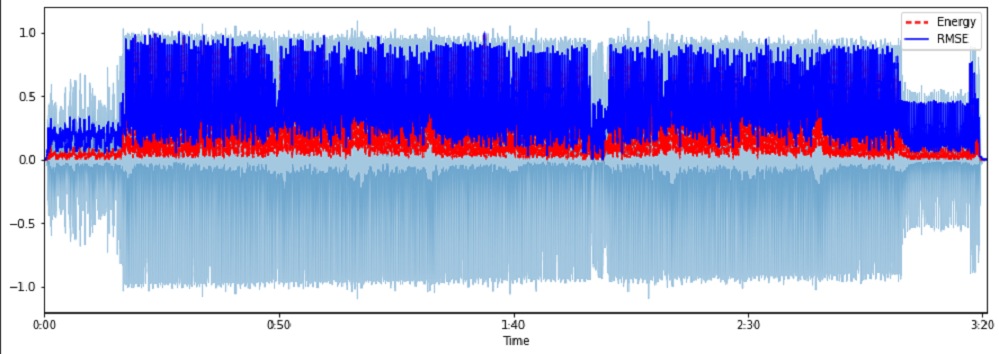
\includegraphics[scale=0.5]{2.png}
        \caption{\lr{Root Mean Square Energy, Signal in Time Domain, and Energy for one song}  }  
    \end{figure}

ج)  آنتروپی شانون:  معیاری برای نشان دادن میزان اطلاعاتی که در سیگنال وجود دارد.\\

\subsection{ویژگی‌های حوزه فرکانس}

اندازه طیف سیگنال، فوریه کوتاه مدت از کروما \lr{ (Chroma-STFT) }\\

 اندازه طیف سیگنال: طیف سیگنال نشان دهنده میزان انرژی در حوزه فرکانس است، به عبارت دیگر میتوان ازین مقدار متوجه شد که در هر فرکانس به خصوص چه میزان انرژی وجود دارد.\\
 فوریه کوتاه زمان\lr{ STFT}  در این تبدیل همانطور که در بالا تر اشاره شد، سیگنال حوزه زمان را به فریم های کوتاه مدت تقسیم میکنیم و از هر فریم تبدیل فوریه میگیریم. با اینکار میتوان یک دید زمان\lr{ –} فرکانس به سیگنال داشت. برای مشاهده بهتره اسپکتروگرام یک موسیقی در شکل زیر به همراه \lr{RMS} رسم شده است.\\
 
        \vskip2cm
 
\begin{figure}[h!]
        \centering
        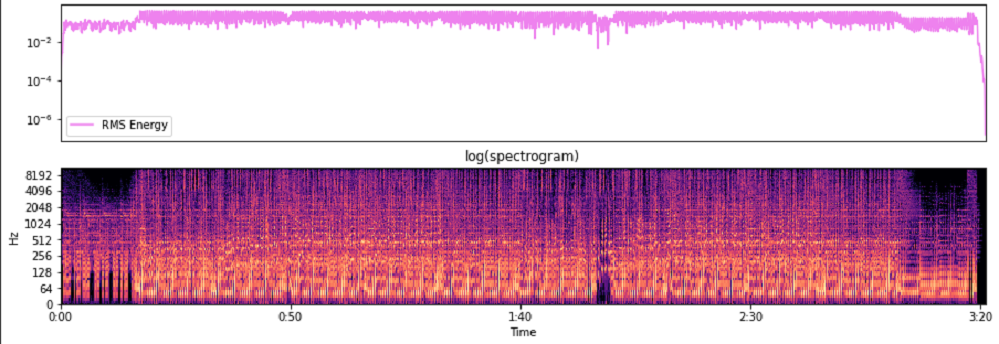
\includegraphics[scale=0.5]{3.png}
        \caption{\lr{Log Power Spectrogram and RMS Energy, As we can see Spectrogram gives us a intuition in both frequency and Time Domain while RMS Energy is only in Time Domain.}  }  
    \end{figure}

\lr{STFT}  میانگین \lr{(mean)}
و چولگی \lr{(skewness)}آن را به فیچرها اضافه میکنیم چرا که میتواند نشان دهنده تمپو سیگنال ما باشد. در شکل زیر \lr{Spectral Centorid} یا همان میانگین اسپکترال برای هر فریم و هچنین رسم شده است.\\
\begin{figure}[h!]
        \centering
        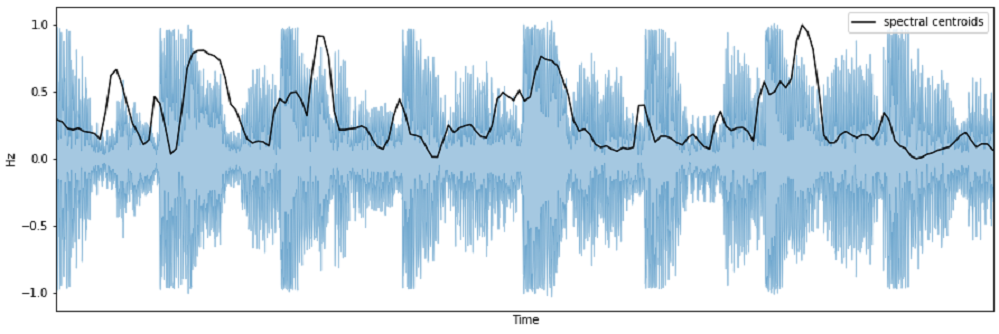
\includegraphics[scale=0.5]{4.png}
        \caption{\lr{Spectral Centroids and Time Domain Music.}  }  
    \end{figure}
    \\
    \begin{figure}[h!]
        \centering
        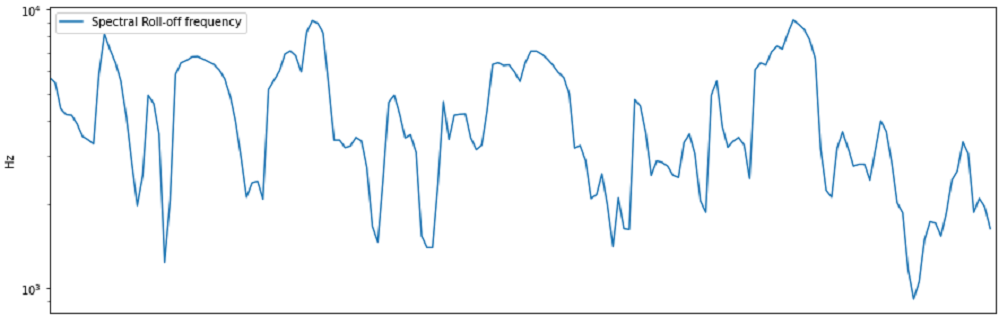
\includegraphics[scale=0.5]{5.png}
        \caption{\lr{Spectral Centroids and Time Domain Music.}  }  
    \end{figure}
    
\lr{Chroma STFT}  :  کروما در حقیقت نگاه به موسیقی از دید 12 \lr{pitch}  میباشد. ابزاری قوی برای تحلیل موسیقی میباشد و به طور معنا داری به ۱۲ سطح با گام مساوی تقسیم میکند. میتواند ویژگی هارمونیکی موسیقی را در خود نمایش بدهد.\\

\begin{figure}[h!]
        \centering
        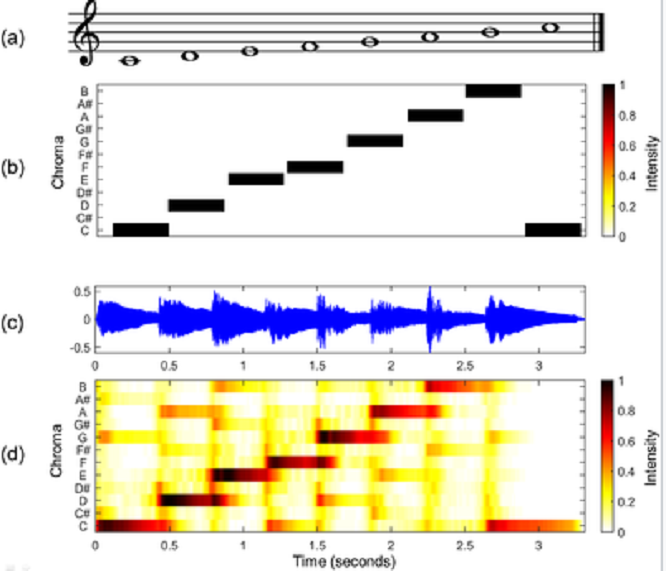
\includegraphics[scale=0.55]{6.png}
        \caption{\lr{Chroma Feature}  }  
    \end{figure}

در شکل 8 توان اسپکتروگرام کروما برای یک موسیقی به مدت 4 ثانیه به نمایش گذاشته شده است.\\
 \begin{figure}[h!]
        \centering
        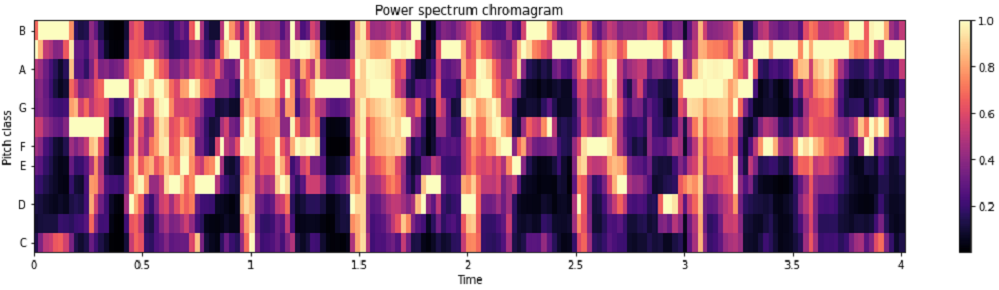
\includegraphics[scale=0.5]{7.png}
        \caption{\lr{Power Spectrum Chromogram, We can See How diffrent Pitches have diffrent powers.}  }  
    \end{figure}
\\

\subsection{ضرایب کپسترال مبتنی بر فرکانس مل}

روشی است برای به دست آوردن ویژگی های صوتی انسان، اگر موسیقی بی کلام باشد نمیتواند ویژگی های خوبی به دست آورد اما در غیر این صورت عملکرد بسیار خوبی دارد.\\ 
\begin{figure}[h!]
        \centering
        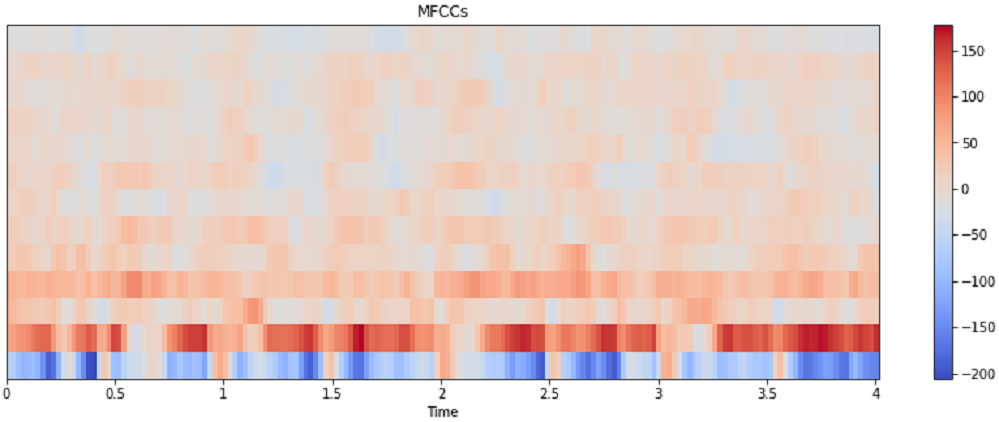
\includegraphics[scale=0.5]{8.png}
        \caption{\lr{MFCC for clipped audio Signal}  }  
    \end{figure}
    \\
    حال با محاسبه همه ویژگی های فوق به وسیله کتابخانه های \lr{librosa} و \lr{surfboard}  میتوان از ویژگی ها استفاده کرد. اما  با توجه به اینکه ما هر آهنگ را به فریم های 50 میلی ثانیه تبدیل میکنیم و حدود 1000 آهنگ داریم و هر آهنگ به طور متوسط 3 دقیقه طول دارد منوجه میشویم که تعداد فیچر ها عددی بسیار بزرگ میشد، برای ذخیره کردن بیشترین اطلاعات ممکن را از فریم های تبدیل شده، میتوان نماینده هایی را مانند میانگین، واریانس، فاصله چارک اول و سوم و چولگی آن را انتخاب کنیم. لازم به ذکر است که این چهار نماینده برای همه ی چهار ویژگی استفاده نشده و به نسبت اهمیت استفاده شده است.\\
    \begin{figure}[h!]
        \centering
        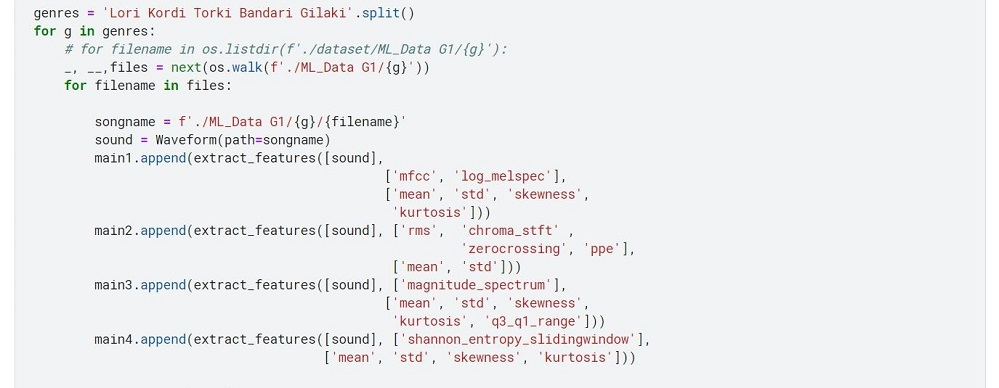
\includegraphics[scale=0.45]{9.jpg}
    \end{figure}
    
\\
فیچر های فوق به وسیله کد بالا به دست می آید. حال بعد از اجرای برنامه متوجه می شویم که برخی از داده ها نرخ نمونه برداری برای سازگاری با کتاب خانه های ما را ندارند در نتیجه باید پاکسازی شوند. آهنگ های زیر حذف شده اند.
\\
\\
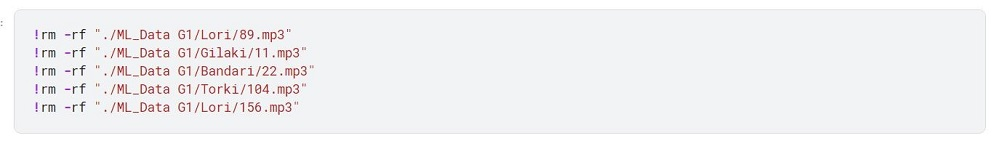
\includegraphics[scale=0.55]{10.jpg}
\\
در مرحله بعد متوجه میشویم که برخی از ویژگی ها حاوی \lr{NaN}  میباشد. میتوان به کمک کتابخانه \lr{scickit learn}  این ویژگی ها را با میانه آن ها جایگزین کرد.\\

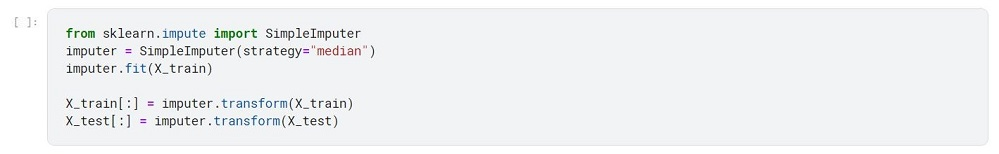
\includegraphics[scale=0.6]{11.jpg}
\\
حال که ویژگی ها استخراج شده اند میتوان بهترین هایشان را برای آموزش \lr{classifier} انتخاب کرد.\\

\subsection{انتخاب ویژگی ها}
برای انتخاب ویژگی دو روش کلی وجود دارد \lr{wrapper methods} و \lr{filter methods} استفاده کرد. با اعمال \lr{PCA} و \lr{LDA} که جزوی از \lr{Filter method} ها هستند مشاهده می‌کنیم که نه تنها عملکرد طبقه‌بند بهتر نمی‌شود که به شدت بدتر می‌شود برای جست‌وجوی علت این پدیده می‌توان به روش انتخاب ویژگی در این دو الگوریتم توجه کرد. الگوریتم \lr{PCA}  سعی در حفظ هرچه بیشتر \lr{variation} در داده‌ها می‌کند و این کار را با انتخاب بردار ویژه‌هایی که متناظر با بزرگترین مقدارهای ویژه هستند انجام می‌دهد که این را می‌توان به پایین بودن \lr{SNR} (نرخ سیگنال به نویز) نسبت داد زیرا بیشترین \lr{variation} هم شامل نویز می‌شود و هم شامل سیگنال که تاثیر بالای نویز در این \lr{variation} باعث عملکرد ضعیف مدل می‌شود.  به عبارت دیگر \lr{PCA}  زمانی میتواند خوب عمل کند که \lr{PC} های انتخاب شده بتواند \lr{variation}  داده ها را به خوبی بپوشاند اما در مورد ما نمیتواند.
\\
با استفاده از \lr{Wrapper Method} ها دقت طبقه‌بند به صورت کلی بهبود می‌یابد که این نکته را به طور کلی می‌توان به این نسبت داد که این روش‌ها مجموعه‌‌ی ویژگی‌ها را تا جایی انتخاب می‌کنند که عملکرد بهبود بیابد و این که این روش‌ها به طور کل بود یا نبود یک ویژگی را مد نظر میگیرند که این روش به نویز مقاوم تر است، هر چند عمومیت (\lr{Genrality} ) کمتری نسبت به \lr{filter methods}  دارند و همچنین از لحاظ پیچیدگی زمانی نیز بد تر است اما نتیجه بهتری را میدهد. در این راستا 1034 فیچر که بهترین عملکرد را داشتند انتخاب شدند.   
	خروجی متناظر بعد از اعمال کردن روش های فوق با الگوریتم های متفاوت در قسمت بعد  مشاهده می شود. 





\pagebreak
\section{طبقه‌بندی}
 در این بخش، ما به منظور طبقه‌بندی موسیقی‌های محلی از سه مدل مختلف  پرسپترون چندلایه، \lr{XGBoost}  و \lr{SVM} استفاده کردیم و هر کدام از مدل‌ها را براساس داده‌های پیش‌پردازش شده آموزش می‌دهیم و در نهایت به تحلیل و بررسی نتایج بدست آمده از این روش‌ها می‌پردازیم و  نتایج را در قالب نمودارهایی ارائه می‌دهیم. 
 \\
\subsection{طبقه‌بندی به کمک شبکه \lr{MLP}:}

در این قسمت، هدف ما این است که براساس ویژگی‌های انتخاب شده یک، یک مدل پرسپترون چند لایه را آموزش بدهیم. به منظور ایجاد این مدل ما از کتابخانه‌ی\lr{Pytorch}  استفاده کرده‌اییم و لازم است که پیش بیان نتایج بدست آمده، توضیحات مختصری در مورد تعداد لایه‌های استفاده شده و پارامترهای به کار گرفته شده بیان گردد.\\
لازم به ذکر است که ما از بین اهنگ‌های موجود ده درصد را برای تست و ده درصد را بیان اعتبار سنجی و هشتاد درصد را به منظور آموزش درنظر گرفتیم. \\
		شمای کلی مدل مورد استفاده: \\
    برای این قسمت، با توجه به حجم بالای ویژگی‌های استخراج شده، ما از کتابخانه \lr{Sklearn} و تابع \lr{SelectFromModel} به منظور انتخاب ویژگی‌های مناسب استفاده کردیم و تخمینگر را براساس الگوریتم \lr{SVM} با پارامتر \lr{C = 0.02}  قرار دادیم بعد از اعمال این الگوریتم از میان ویژگی‌های موجود، 366 ویژگی پراهمیت انتخاب شد که ادامه‌ی کار را براساس این ویژگی‌ها انجام می‌دهیم. \\

اکنون پس از آماده سازی مجموعه داده، به توضیح مدل ساخته شده می‌پردازیم، ما در این مدل در لایه اول به تعداد ویژگی‌های انتخاب شده یعنی 366نورون قرار می‌دهیم، در لایه دوم و سوم به ترتیب ده و بیست نورون قرار داده و لایه آخر به این دلیل که وظیفه‌ی ما دارای 5 برچسب است، از 5 نورون استفاده می‌کنیم تا در نهایت نورون که بالاترین مقدار را داشت نشان دهنده‌ی نوع موسیقی باشد. لازم به ذکر است که در میان این شبکه‌ها ما از لایه‌های \lr{drop out}  به منظور پیشگیری از \lr{overfit} استفاده کرده‌اییم. همچنین تابع فعالساز مورد استفاده در لایه دوم و سوم \lr{Relu}  و در لایه‌ی آخر از \lr{LogSoftmax}  استفاده شده است.\\ 
در شکل 9 شمای کلی شبکه مورد استفاده نشان داده شده است.\\
  
\begin{figure}[h!]
        \centering
        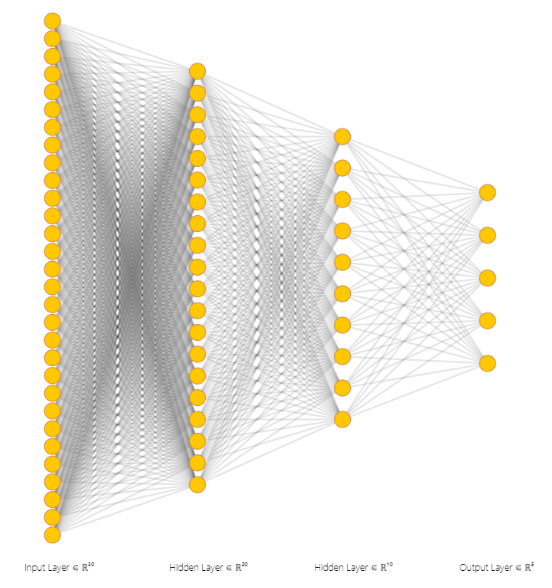
\includegraphics[scale=0.55]{b.png}
        \caption{\lr{MLP Structure}  }  
    \end{figure}


	پارامترها و الگوریتم بهینه‌سازی استفاده شده:\\

به منظور انجام این وظیفه ما مقدار \lr{drop out}  را برابر 50 درصد درنظر گرفته‌ایم  همچنین با توجه به ماهیت که تابع هزینه مورد استفاده \lr{Cross Entropy}  می‌باشد. تابع بهینه‌سازی مورد استفاده نیز \lr{Adam} است که نرخ یادگیری آن را 0.0001 در نظر گرفتیم و در مجموعه ما یادگیری را در 500 \lr{Epoch} انجام می‌دهیم.\\
پس از بیان این مقدمات اکنون لازم است که در خصوص نتایج بدست آمده توضیحات بیان گردد.\\
	نتایج بدست آمده و تحلیل‌ها:\\

همانطور که بیان شد ما آموزش را در 500 ایپاک و تا زمانی که بیش‌برازش رخ ندهد ادامه دادیم و در نهایت نمودار مربوط به میزان \lr{loss} بدست آمده برای دو داده‌ی اعتبارسنجی و آموزش نسبت به تعداد ایپاک‌ها مطابق شکل زیر شد. همانطور که در این نمودار به وضوح مشخص است، با افزایش ایپاک‌ها مقدار \lr{Loss} در هر دو داده‌ با کاهش همراه است و این نکته به وضوح مشخص است که الگوریتم ما به هیچ وجه دچار بیش‌برازش نشده است و در جایی که روند کاهشی به یک روند پایدار تبدیل شد و ما آموزش را متوقف کردیم. \\
  
\begin{figure}[h!]
        \centering
        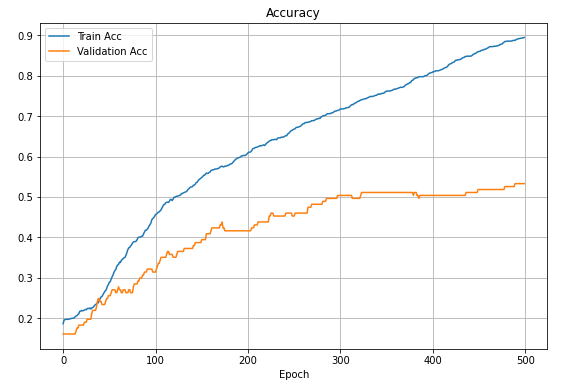
\includegraphics[scale=0.5]{c.png}
        \caption{\lr{Loss function}  }  
    \end{figure}
  
\begin{figure}[h!]
        \centering
        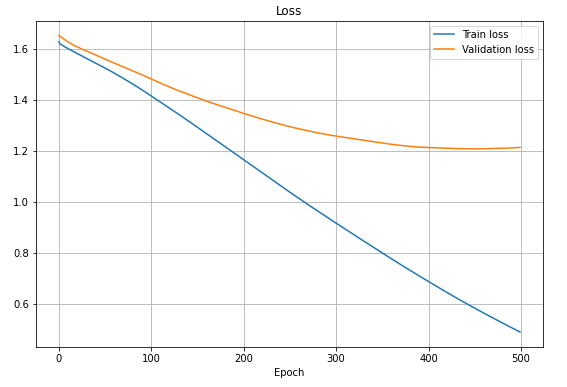
\includegraphics[scale=0.5]{d.png}
        \caption{\lr{Accuracy}  }  
    \end{figure}

اکنون به منظور بررسی عملکرد کار، یک نمودار براساس میزان دقت بدست آمده در هر ایپاک برای دو داده‌ی اعتبارسنجی و آموزش رسم کرده‌اییم. همانطور که در این نمودار مشخص است، دقت داده‌‌های آموزش تا حدود 90 درصد می‌رسد اما دقت داده‌های اعتبارسنجی در این 500 ایپاک بیشتر از 55 درصد نمی‌شود. \\

پس از پایان مرحله‌ی آموزش مدل، اکنون مدل توسط داده‌های آموزش مدل آزمایش قرار می‌گیرد. به این منظور داده‌های تست موجود را به ورودی مدل اعمال کرده و پیش‌بینی نوع آهنگ‌های برآن اساس صورت می‌گیرد و با توجه به برچسب اصلی داده‌های معیارهای دقت و \lr{F1 score(macro)}  برای نتایج بدست آمده محاسبه می‌شود.\\ 
که نتایج آن مطابق جدول زیر است:\\

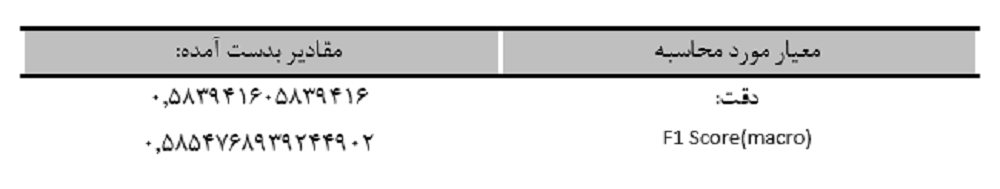
\includegraphics[scale=0.45]{e.png}
\\
دقت و \lr{f1}  بدست آمده چیزی نزدیک به 60 درصد می‌باشند که باتوجه به نوع ماهیت وظیفه و همچنین نوع شبکه‌ی استفاده شده تقریبا می‌توان بیان داشت که عملکرد به نسبت خوبی ارائه شده است. شاید بتوان کمی از عملکرد ضعیف بدست آمده را بدلیل شباهت‌هایی که بین برخی از آهنگ‌ها بوده است بیان کرد، که این شباهت‌ها سبب شده‌اند مدل به خوبی نتواند انواع مختلف موسیقی‌ها را تمایز دهد.  به عنوان مثال در برخي از اهنگ‌هاي محلي خواننده به زبان محلي خود در يك سبك خاص موسيقيايي آهنگ خود را خوانده است و در صورتي كه يك خواننده ديگر با زبان محلي ديگر در همان سبك موسيقي آهنگي را خوانده باشد هر چند كه نوع زبان خواننده متفاوت است. اما ميتواند اين موضوع در خطاي مدل ما تاثير گذار باشد. شايد بتوان بيان كرد به منظور کاهش این خطاها باید ویژگی‌هایی را صرفا براساس صدای خواننده استخراج کرد تا بتواند تمایز بیشتری را در این وظیفه که دسته‌بندی موسیقی‌های محلی است ایجاد کند و دقت مدل افزايش يابد. همچنين حتي می‌توان با این داده‌ها توسط شبکه‌های پیچیده‌تر دیگری مانند \lr{CNN} یا \lr{LSTM} به دقت‌هاي نسبتا بالاتری دست پیدا کرد. 
اما در پایان این بخش یک نمودار \lr{Confusion matrix}  براساس نتایج به دست آمده در شکل زیر رسم شده است.\\ 
همانطور که در این نمودار مشخص است، محور افقی تعداد آهنگ‌های پیش‌بینی شده در هر دسته را نشان می‌دهد و هر چه مقادیر موجود در قطر اصلی این ماتریس کمرنگ تر باشد نشان دهنده‌ی عملکرد مناسب مدل ایجاد شده در پیش‌بینی آهنگها  می‌باشد. \\

\begin{figure}[h!]
        \centering
        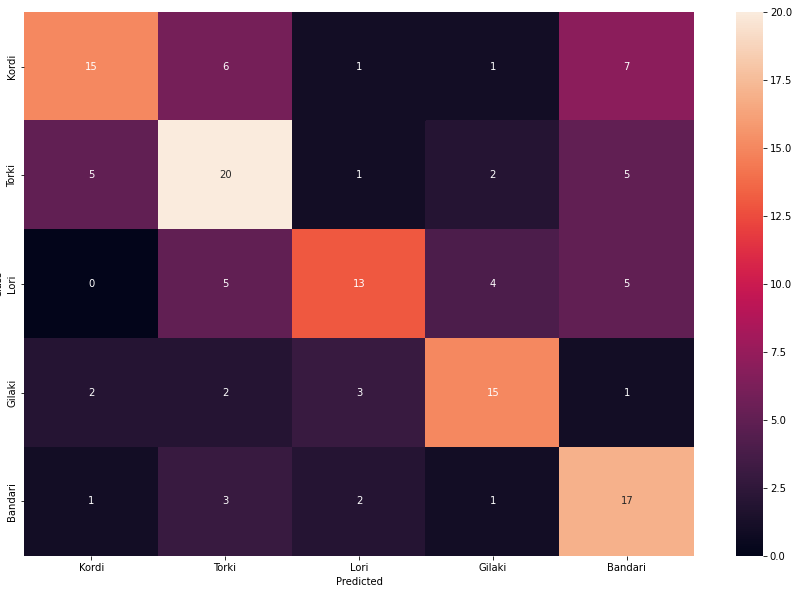
\includegraphics[scale=0.5]{f.png}
        \caption{\lr{Confusion Matrix For MLP Classifier}  }  
    \end{figure}

\\
براساس این نتایج به وضوح مشخص است که، عملکرد مدل تقریبا در دسته‌بندی موسیقی‌ها مناسب بوده است و مدل بهترین عملکرد را در موسیقی ترکی داشته است و توانسته است بخش زیادی از موسیقی‌ها این دسته‌ را به درستی تشخیص دهد و عملکرد این مدل در تشخیص موسیقی لری به نسبت سایر موسیقی‌ها کمی نامناسب‌تر بوده است.\\ 
به طور کلی می‌توان دلیل این ضعف را هم در ماهیت داده‌ها به دلیل شباهت برخی موسیقی‌ها( از لحاظ سبک موسیقیایی، زبان خواننده و... )، شبکه‌ی عصبی استفاده شده(شبکه \lr{MLP} )که مدل خیلی پیچیده‌ای براین وظیفه نیست و هم ویژگی‌های موجود که شاید براساس نوع وظیفه آنچنان مناسب آن نباشند بیان کرد.\\ 


\subsection{طبقه‌بندی به کمک شبکه \lr{XGBoost}:}

\lr{XGBoost} یک طبقه بند از دسته‌ی  \lr{ensemble learning} است که به طور کلی از نرکیب چندین و چند مدل ضعیف‌تر و قرار دادن آن‌ها به صورت موازی یا سری به یک طبقه‌بند قوی‌تر می‌رسد. یک درخت تصمیم که واحدهای سازنده‌ی جنگل‌های تصادفی هستند در هر مرحله از عمقشان فضا را با استفاده از تنها یک ویژگی به دو قسمت تقسیم می‌کنند و با عمق بیشتر افرازهای بیشتر و قوانین طبقه‌بندی بیشتری را ایجاد می‌کنند. درخت‌های تصمیم به دلیل ساختار ساده‌ی خود معمولا دقت پایینی دارند و نتیجه‌ی خوبی در دنیای واقعی کسب نمی‌کنند اما سازندگان الگوریتم ماشین‌لرنینگ با استفاده از اصل خرد جمعی(با رای‌گیری از تعداد افراد بسیار زیاد خطا به نسبت کم می‌شود) به این نتیجه رسیدند که هر بار درخت‌ها را با قسمت محدودی از ویژگی‌ها آموزش دهند و در نهایت از بین تمام آن‌ها رای‌گیری کنند. مشکل اصلی این الگوریتم این است که درخت‌ها از اشتباهات یکدیگر نمی‌آموزند و عملا به درخت‌ها به صورت مستقل نگاه می‌شود. روش‌های \lr{boosting} برای حل این مشکل به وجود آمدند.  در روش‌های \lr{boosting} درخت‌ها به جای این که در توازی یکدیگر باشند با یکدیگر سری هستند و هر درخت روی خطای درخت قبلی آموزش می‌بیند. روش‌های مبتنی بر گرادیان به این نحو عمل می‌کنند که درخت‌های بعدی هم‌جهت با تابع گرادیان ویژگی‌های قبلی حرکت می‌کنند. \lr{Xgboost} یک پیاده‌سازی موازی از الگوریتم‌های مبتنی بر گرادیان است.

\begin{figure}[h!]
        \centering
        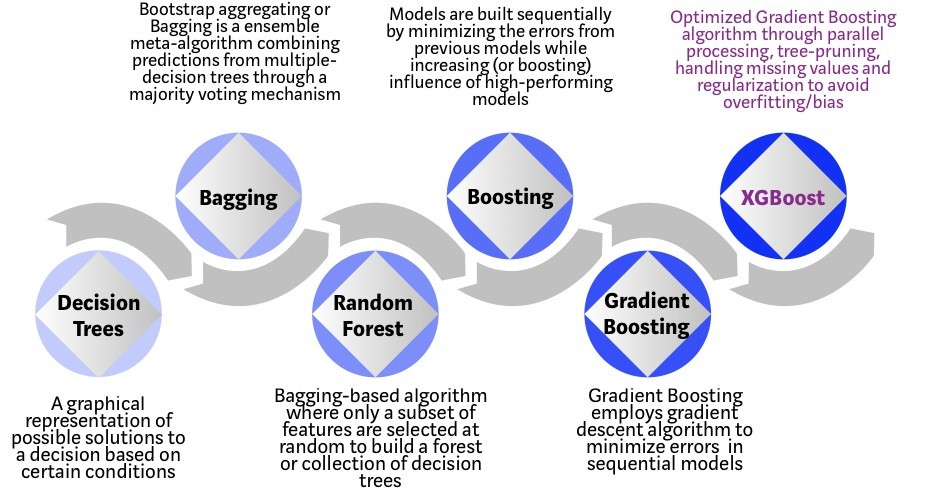
\includegraphics[scale=0.5]{f.jpg}
        \caption{\lr{Evolution of XGBoost Algorithm from Decision Trees}  }  
    \end{figure}

ما در طبقه‌بندی خود از روش \lr{xgboost} به دلیل انعطاف بالای آن در جذب اطلاعات استفاده کردیم، که به دلیل تعداد داده‌های محدود پیش‌بینی می‌شد که مدل به داده‌های آموزش چسبنده شود که نتایج این نکته را تایید می‌کرد اما نکته‌ی بسیار قابل توجه این است که این چسبندگی باعث عدم عمومیت‌بخشی نشد و این الگوریتم از تمام الگوریتم‌های دیگر بر روی داده‌ی ارزیابی عملکرد بهتری داشت.  عکس های زیر گفته های ما را تایید میکند، با توجه به اینکه \lr{Cross-Validation Score}  همواره با افزایش نمونه ها در حال افزایش است، میتوان نتیجه گیری کرد که مدل تشنه داده است.
برای درک بهتر باید مد نظر داشته باشیم دو منبع خطا به طور کلی وجود دارد:
الف) اشتباه در فرض اولیه برای مدل
ب) کم بودن تعداد داده ها برای ابعاد مسئله

\begin{figure}[h!]
        \centering
        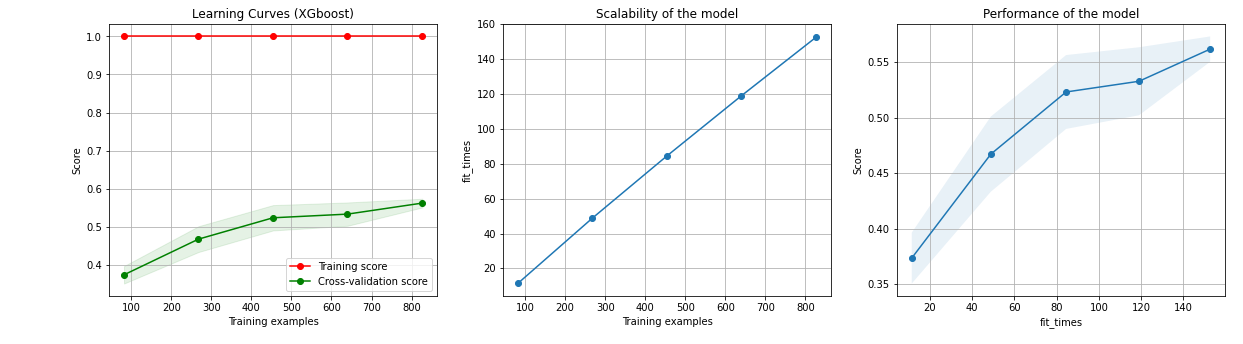
\includegraphics[scale=0.4]{g.png}
        \caption{\lr{Learning Curves, Scalability of Model, Performance of the model by fit times; as we can see variation of model performance and Cross-Val Score has been shown.}  }  
    \end{figure}

حال با توجه به نمودار های شکل ۱۴ و دقتی که برای مدل به دست آوردیم می توان نتیجه گرفت که در 
مدل ساخته خطای "ب" جلوگیری میکند از عملکرد بهتر مدل. در نهایت عملکرد مدل را نیز میتوان مشاهده کرد به ازای فیچر های مختلف:


\begin{figure}[h!]
        \centering
        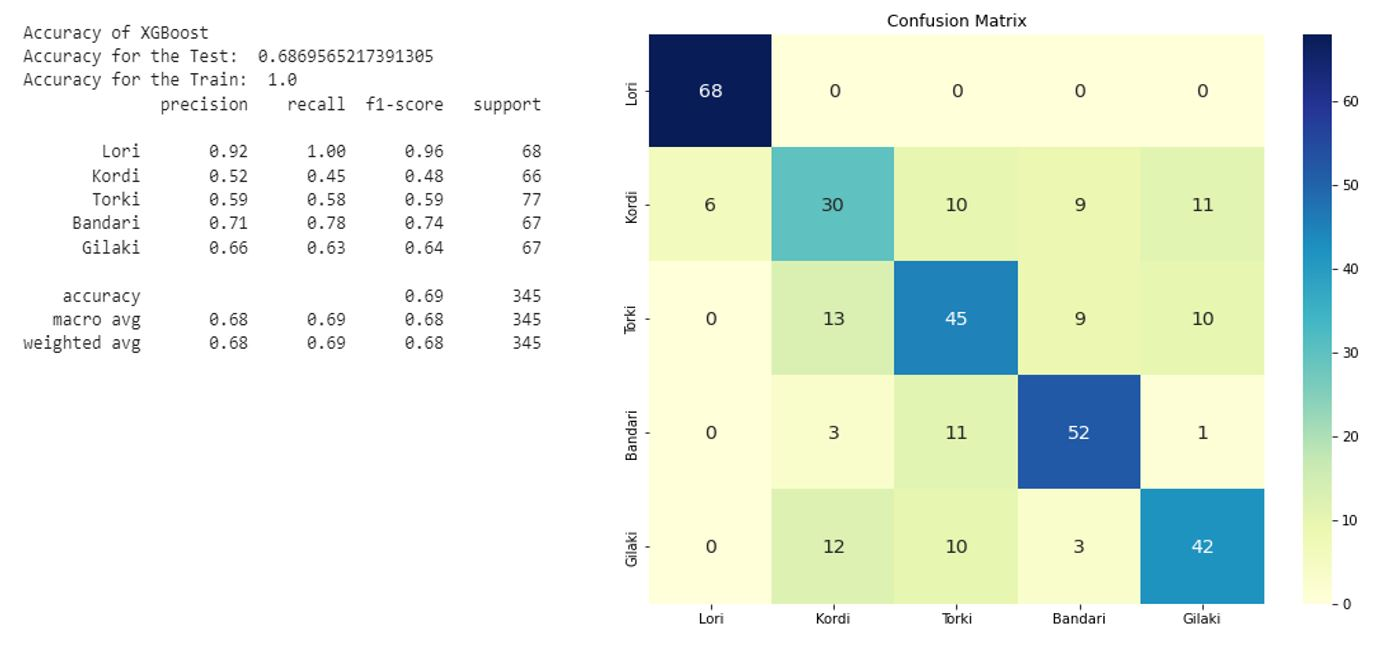
\includegraphics[scale=0.35]{h.JPG}
        \caption{\lr{Accuracy of XGboost for Raw Data and Confusion Matrix}  }  
    \end{figure}

با توجه نتایج مشاهده میکنیم که در دو کلاس لری و بندری با توجه به ریتیمی که دارند خطای کمتری وجود دارد اما در کلاس کردی،با توجه به این نکته که آهنگ های کردی از لحاظ ریتم و موسیقی همه طیف ها را در خود دارد در نتیجه بیشترین خطا را دارد. 
اما در مورد خطا متوجه میشویم که به داده های آموزش \lr{over fit} شده است و برای حل مشکل دو راه وجود دارد، استفاده از مدل ساده تر و افزایش نمونه ها. در نمودار \lr{cross val score}   و توضیحات آن گفته شد که اضافه کردن داده به مدل میتواند راه حل مناسب تری باشد.


\begin{figure}[h!]
        \centering
        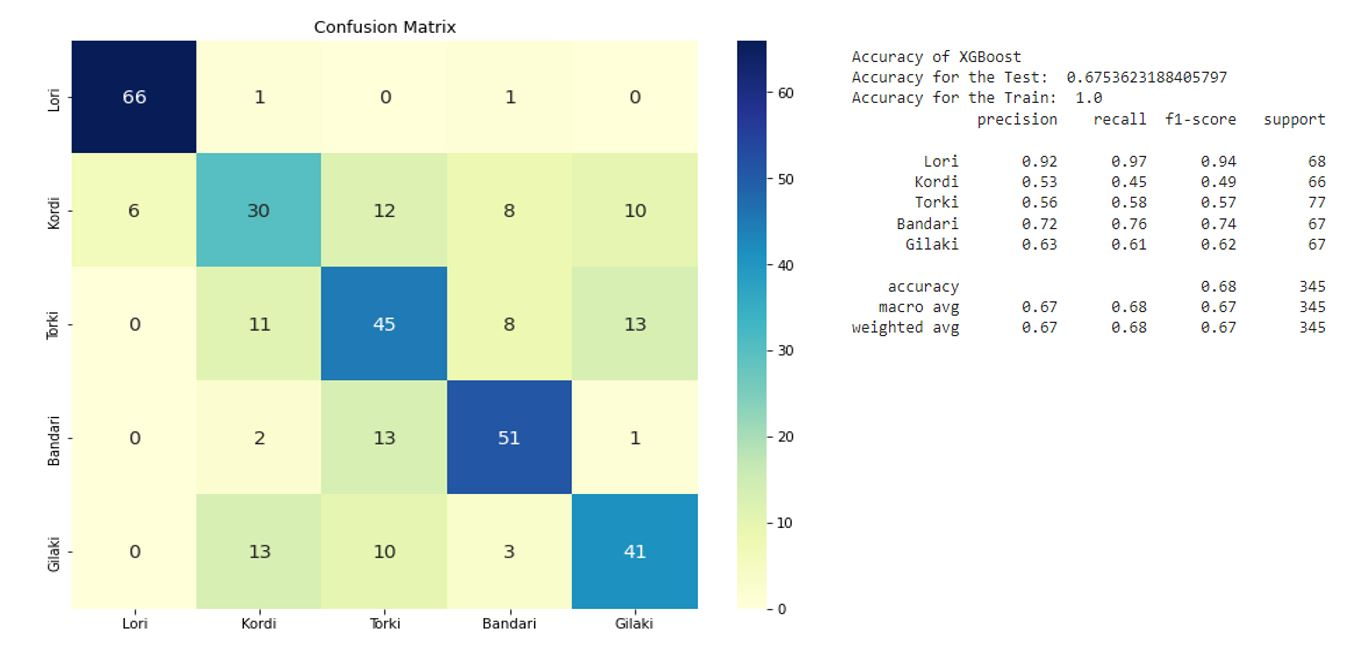
\includegraphics[scale=0.35]{i.JPG}
        \caption{\lr{XGBosst With Feature selection (Wrapper Methods) Results}  }  
    \end{figure}
    \\
همانطور که در بخش اتخاب فیچر ها گفته شد، انتخاب ویژگی ها و کاهش آن ها باعث عمکرد مناسب مدل میشود اما به طور کلی باعث افزایش دقت نشد چرا که میزان سیگنال به نویز مقدار کمی است.
اگر  \lr{XGboost}  را به ویژگی های به دست آمده با \lr{PCA} اعمال کنیم همانطور که گفته شد نتایج گرفته شده بسیار بد می باشد و فیچر های اشتباه به عنوان \lr{Principal Component}  انتخاب میشوند.

\begin{figure}[h!]
        \centering
        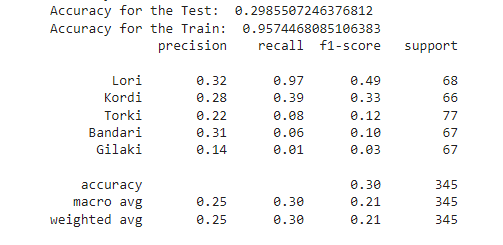
\includegraphics[scale=0.5]{j.png}
        \caption{\lr{Report for XGBoost Classifier after Performing PCA on data}  }  
    \end{figure}

تنها نکته امیدوار کننده راجب این طبقه بند کاهش چسبندگی آن به داده های آموزش است اما با توجه به دقت داده های تست خروجی ها اصلا قابل قبول نیستند.


\subsection{طبقه‌بندی به کمک شبکه \lr{SVM}:}

مدل آخری که استفاده شده است \lr{SVM}  
است که نتایج آن در این قسمت آمده است.\\
با  استانداردایز کردن داده ها و سپس اعمال \lr{SVM}، میتوان نمودار های یادگیری \lr{(learning curve )} میتوان و \lr{Cross Val Score} را مشاهده کرد. با توجه به اینکه بعد از 600 نمونه آموزشی \lr{Score}  کاهش یافته است میتوان نتیجه گرفت که اگر نمونه ها زیاد شود دیگر عملکرد مدل بهتر نمی شود. به عبارت دیگر مدل بایاس دارد و به اندازه کافی \lr{Variation} داده ها را نمیتواند پوشش دهد.


\begin{figure}[h!]
        \centering
        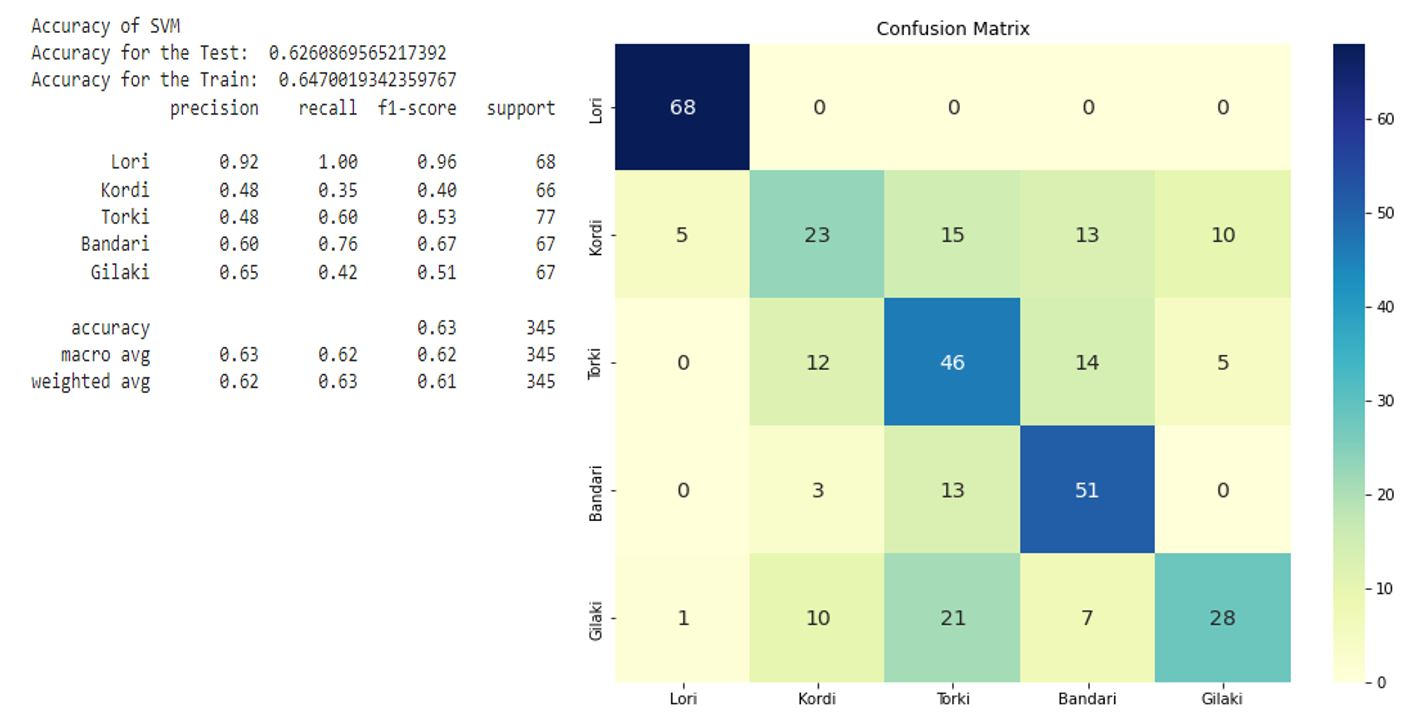
\includegraphics[scale=0.35]{k.JPG}
        \caption{\lr{Confusion and report For SVM on Standardized Features}  }  
    \end{figure}

\begin{figure}[h!]
        \centering
        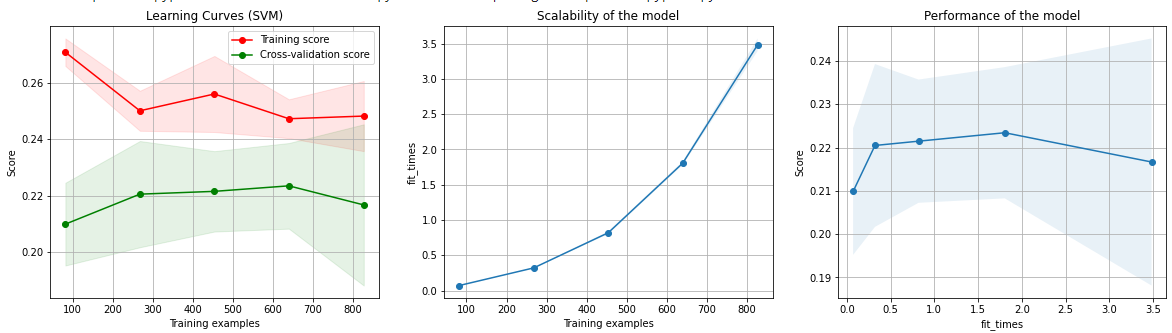
\includegraphics[scale=0.4]{l.png}
        \caption{\lr{Learning Curves For SVM}  }  
    \end{figure}

\begin{figure}[h!]
        \centering
        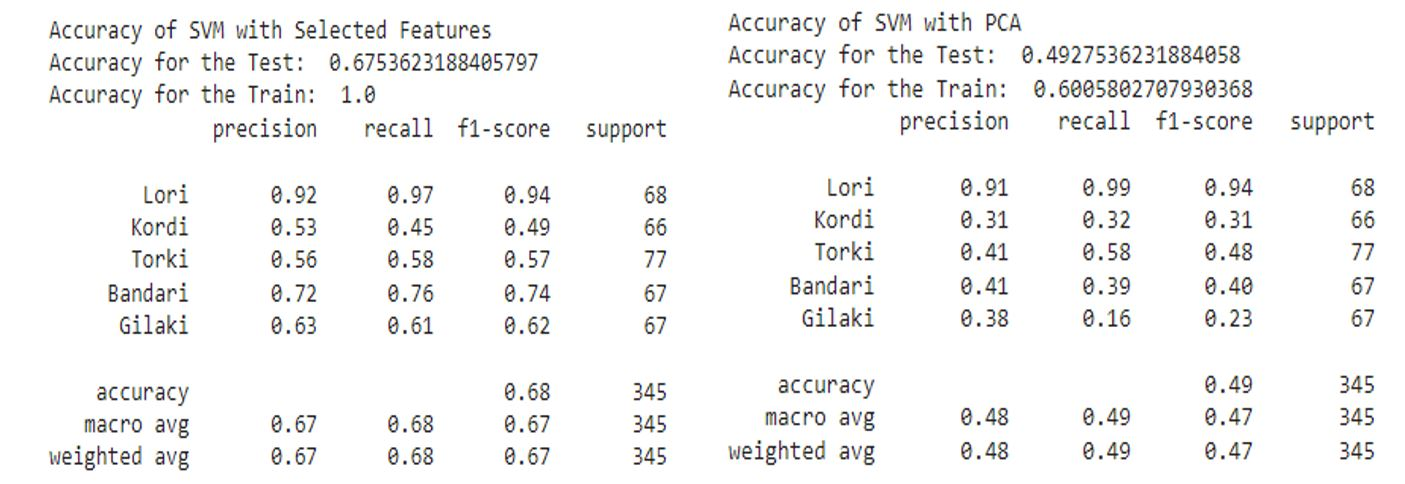
\includegraphics[scale=0.35]{m.JPG}
        \caption{\lr{Report For SVM classifier applied to Features Extracted From SFS(Left) and PCA(right)}  }  
    \end{figure}
با اعمال \lr{PCA}  همانطور که انتظار داشتیم و قبلا توضیح داده شد عملکرد کلی مدل کاهش یافت و با اعمال \lr{SFS}  میتوان مشاهده کرد که عملکرد مدل بهتر شده است اما دچار \lr{Over fitting} شده است که قابل حدس بود چرا که \lr{Objective Function} ما در ابتدا برای انتخاب ویژگی ها  با \lr{SFS} از مدل خطی استفاده کردیم (مشابه \lr{SVM}  است) در نتیجه به شدت ویژگی های ما کمبود \lr{generality} دارند درنتیجه  \lr{overfit} میشود.
\\
\pagebreak
\section{خوشه‌بندی}
\vskip1cm
در این بخش از پروژه، مطابق صورت سوال از ما خواسته شده است که دو الگوریتم مختلف خوشه‌بندی را به ازای سایز خوشه‌های یک تا پنج بر روی داده‌های ورودی اعمال كنيم. در ابتدا‌ی این بخش به منظور این که یک دیدکلی نسبت به داده‌ها داشته باشیم، داده‌ها را در قالب یک نمودار سه‌بعدی نمايش می‌دهیم.  در قدم بعدی داده‌ها را با استفاده از الگوریتم‌های خوشه‌بندی \lr{K-means} و الگوريتم خوشه‌بندي سلسله مراتبي خوشه‌بندی می‌کنیم. در هنگام اعمال الگوريتم \lr{K-means} با استفاده از در یک نمودار تعداد بهینه خوشه‌ها  نمايش می‌دهيم، سپس به ازای هر کدام از خوشه‌های بدست آمده معيارهاي \lr{Purity} ،‌\lr{Rand Index} و \lr{F1}  را محاسبه می‌کنیم و در آخر تحلیلی بر روی نتایج بدست می‌آوریم.
\\
\subsection{استفاده از روش \lr{PCA} برای کاهش ابعاد:}

ابعاد داده بسیار بالا است و درک آن برای ما بسیار سخت است برای این که درک اولیه‌ای از خوشه‌ها داشته باشیم سعی می‌کنیم که آن‌ها را در سه بعد نشان دهیم برای کاهش ابعاد از \lr{Principle Component Analysis} استفاده می‌کنیم. می‌دانیم که \lr{PCA}  روشی است که محورهایی را انتخاب می‌کند که بیشترین واریانس را در خود ذخیره کنند. در نتیجه با اعمال \lr{PCA} و کاهش ابعاد به ۳ به شکل زیر می‌رسیم. توجه کنید که خوشه‌بندی در همان ابعاد اصلی اتفاق افتاده است و صرفا برای مصورسازی به ابعاد پایین‌تر منتقل شده است.
\\

\begin{figure}[h!]
        \centering
        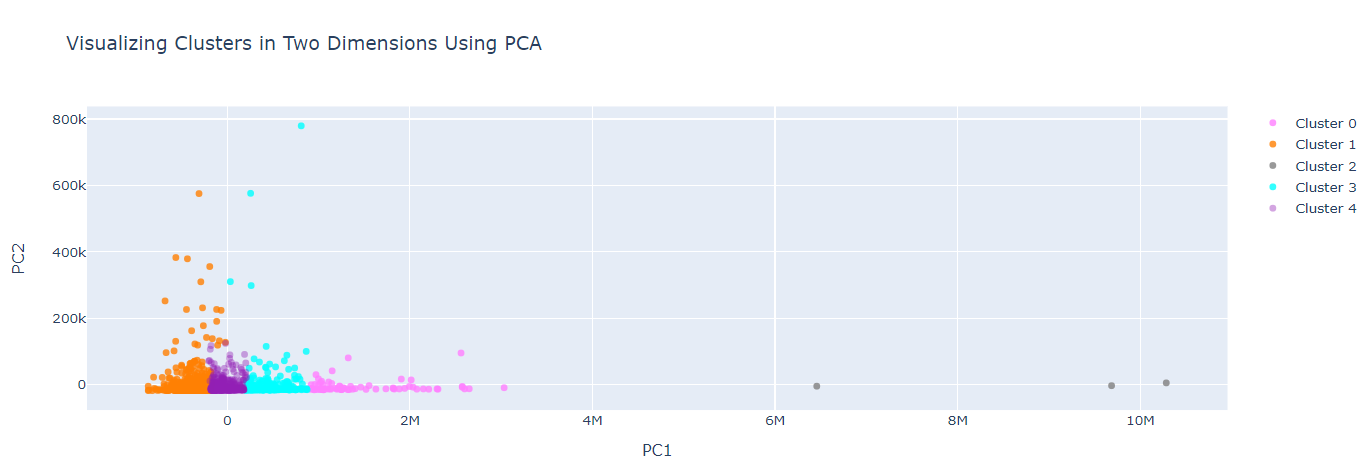
\includegraphics[scale=0.4]{c2.png}
        \caption{\lr{Using PCA for visualizing clustering output in 2 dimensions.}  }  
    \end{figure}
\\
\vskip2cm
\begin{figure}[h!]
        \centering
        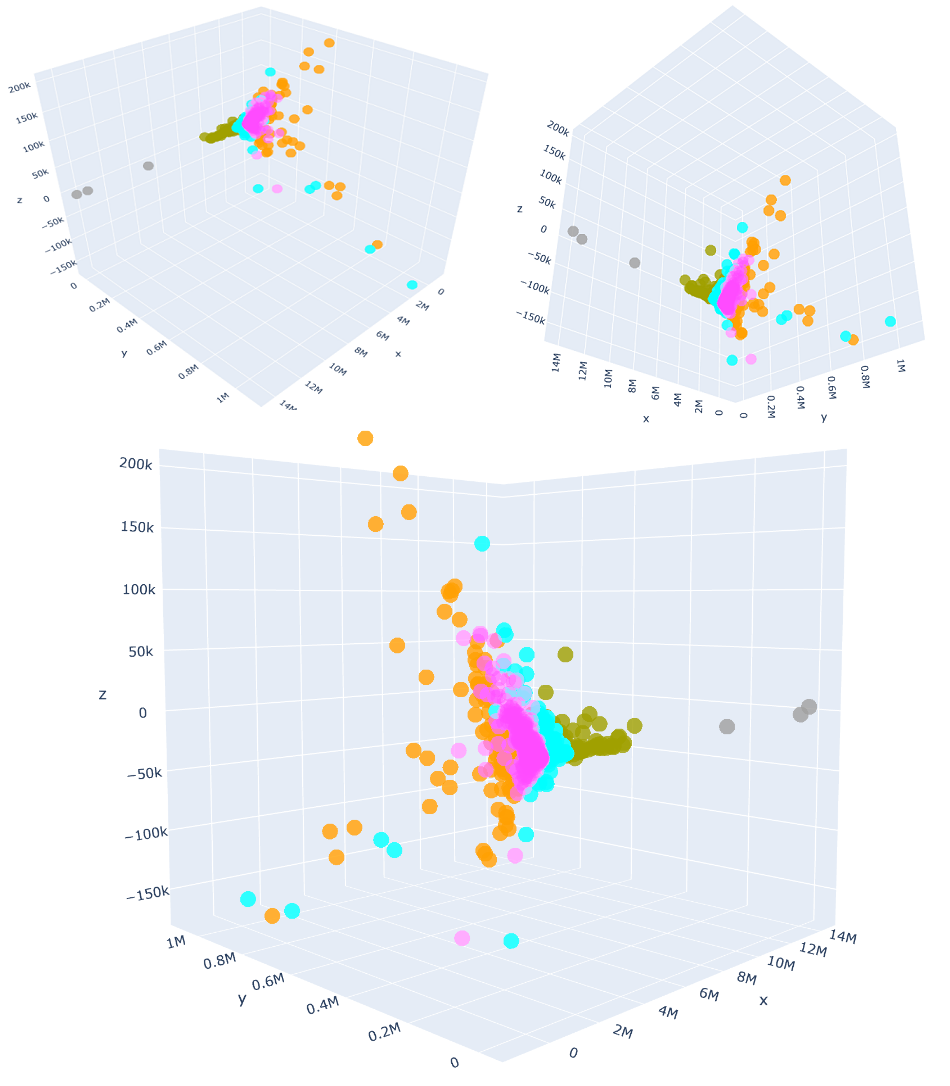
\includegraphics[scale=0.45]{c1.png}
        \caption{\lr{Visulizing by PCA after clustering.}  }  
    \end{figure}
\\

 
\subsection{خوشه‌بندی به روش \lr{k} نزدیکترین مرکز:}

در این قسمت، در ابتدا الگوریتم \lr{K-means} را به عنوان الگوریتم خوشه‌بندی در نظر می‌گیریم و سایز خوشه‌ها را از 1 تا 5 مطابق خواسته‌ی مسئله تغییر می‌دهیم. همچنین ما نمودار مربوط به میزان \lr{Distrotion}  (  میانگین مجذور فواصل از مراکز خوشه‌ها – به کمک فاصله اقلیدسی ) براساس تعداد خوشه‌های یک تا 10  را برای این الگوریتم رسم می‌کنیم که نتایج مربوط به آن مطابق نمودار زير مي‌شود. 
\\

\begin{figure}[h!]
        \centering
        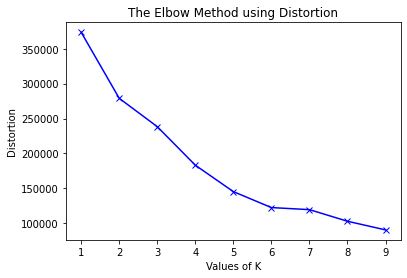
\includegraphics[scale=0.6]{km1.png}
        \caption{\lr{The Elbow Method using Distortion}  }  
    \end{figure}


در این نمودار محور افق تعداد خوشه‌ها و محور عمود   نشان‌دهنده‌ی میزان \lr{Distrotion}  می‌باشد همانطور که در این نمودار مشخص است، نقاطی که در آن‌ها زانو‌هایی رخ‌داده است،‌ نشان‌ دهنده‌ي نقاط مناسب براي تعداد خوشه‌ها مي‌باشد، و همانطور که مشاهده می‌شود در اندازه‌ي خوشه‌ی دو و هفت این زانو‌ها اتفاق افتاده است. (شايان ذكر است به منظور داشتن ديد كامل‌تر ما تعداد خوشه‌ها را در اين بخش تا 10 افزايش داديم اما در تحليل نتايج تعداد خوشه‌ها .را يك تا پنج در نظر گرفتیم)
\\
همچنین ما به منظور ارزیابی نتایج بدست آمده از معیارهای زیر به ازای هر کدام از اندازه‌های خوشه‌ی یک تا پنج محاسبه‌ می‌کنیم. 
معیار اول) شاخص خلوص(\lr{Purity}) است که درصد مطابقت بین برچسب‌های خوشه‌بندی و برچسب‌های واقعی را می‌سنجد( این معیار هر چه به یک نزدیکتر باشد نشان دهنده‌ی کیفیت مناسب خوشه‌بندی است).
\\
معیار دوم) شاخص رند اصلاح شده ( \lr{Rand Index} ) است که میزان شباهت بین دو شیوه‌ی برچسب گذاری را می‌توان با این شاخص اندازه‌ گیری کرد ( این معیار هر چه به یک نزدیکتر باشد نشان دهنده‌ی کیفیت مناسب خوشه‌بندی است).
\\
معیار سوم) \lr{F1 score}  که به این منظور باید مقادیر مثبت صحیح، مثبت کاذب، منفی صحیح و منفی کاذب در این وظیفه‌ی خوشه‌بندی محاسبه شود که ما براساس تعاریفی که برای مقادیر مثبت صحیح، مثبت کاذب و ... در مسئله خوشه‌بندی وجود دارد(در ادامه تعاریف بیان شده است) یک تابع نوشتیم و نتایج را با آن‌ها ارزیابی کردیم.
\\
منظور از مثبت صحیح، آن زوج مشاهداتی هستند که در یک دسته‌ هستند و در یک خوشه نیز قرار گرفته‌اند.
\\
منظور از منفی صحیح، آن زوج مشاهداتی هستند که در دو دسته مجزا هستند و در خوشه مجزا نیز قرار گرفته اند.
\\
مثبت کاذب، آن زوج مشاهداتی است که در دو دسته مجزا قرار گرفته‌اند و در یک خوشه قرار دارند.
\\
منفی کاذب، آن زوج مشاهداتی که در یک دسته‌ قرار دارند و به اشتباه در دو خوشه قرار گرفته‌اند.
\\
اکنون تمامی این معیارها را به ازای اندازه‌ی خوشه‌های یک تا پنج براساس الگوریتم \lr{K-means}  نمایش می‌دهیم در قالب یک جدول نشان میدهیم.
\\

\begin{figure}[h!]
        \centering
        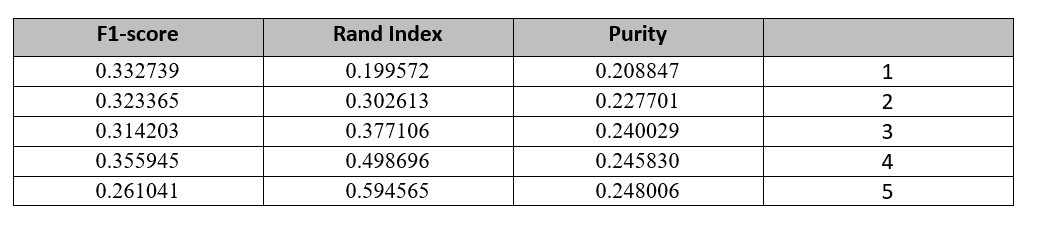
\includegraphics[scale=0.45]{km2.png}
        
    \end{figure}
\\
در ادامه نیز به ازای اندازه‌ی خوشه‌های 3، 4 و 5 ماتریس درهم‌ریختگی رسم می‌شود تا تعداد اهنگ‌های قرار گرفته شده در هر خوشه نمایش داده شود.  
\\

\begin{figure}[h!]
        \centering
        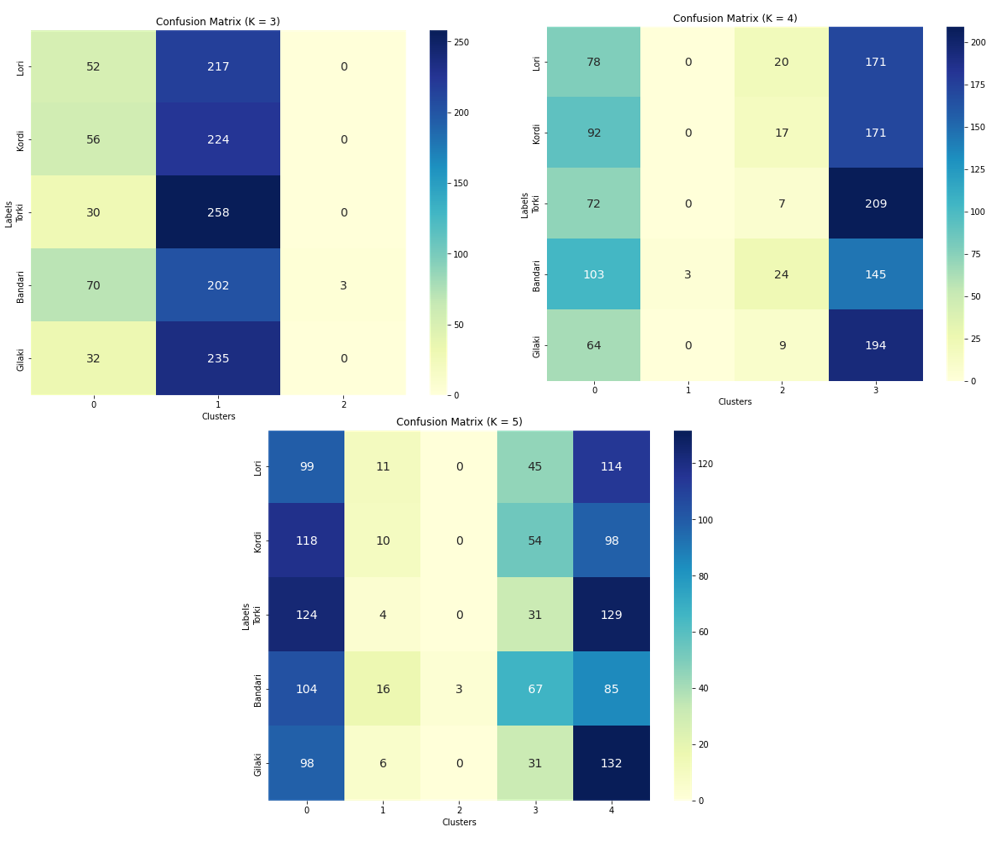
\includegraphics[scale=0.45]{km3.png}
        \caption{\lr{Confusion matrix of K-means clustering}  }  
    \end{figure}

\pagebreak



\subsection{خوشه‌بندی به روش سلسله مراتبی :}

\\
در این بخش نیز نتایج الگوریتم‌ سلسله مراتبی به ازای سایز خوشه‌های یک تا پنج بررسی می‌شود. در جدول زیر معیارها مورد استفاده به ازای هر اندازه‌ی خوشه محاسبه شده است و نمایش داده می‌شود. 
\\
\begin{figure}[h!]
        \centering
        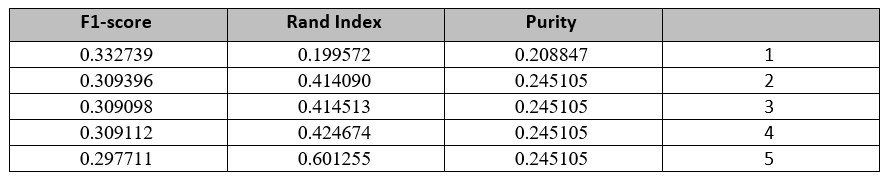
\includegraphics[scale=0.45]{km4.PNG}
        
    \end{figure}
\\
در نمودارهای زیر نیز ماتریس درهم‌ریختگی به ازای سایز خوشه‌های 3 تا 5 نمایش داده‌ می‌شود که تعداد هر دسته‌ از اهنگ‌های قرار گرفته شده در هر خوشه را نمايش مي‌دهد. 
\\

\begin{figure}[h!]
        \centering
        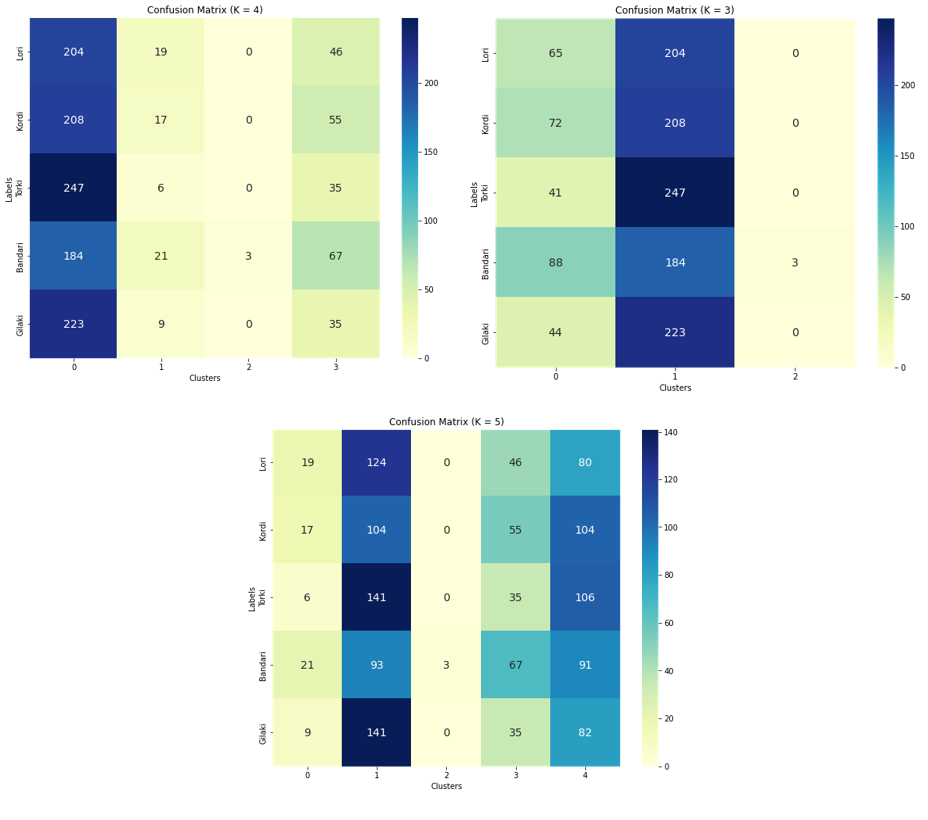
\includegraphics[scale=0.45]{km5.png}
        \caption{\lr{Confusion matrix of Hieratical clustering}  }  
    \end{figure}

\\
اکنون لازم است که پس از نمایش نمودارها و مقادیر بدست آمده برای معیارهای مختلف، به تحلیل این معیارها بپردازیم. همانطور که از نتایج هر دو الگوریتم مشخص است، تقریبا نتایج بدست آمده برای معیارهای در نظر گرفته شده برای هر دو الگوریتم با یکدیگر برابر هستند. اما معیار \lr{Rand Index}  به ازای اندازه‌ی خوشه‌ی 5 در الگوریتم سلسله مراتبی کمی از الگوریتم \lr{K-means}  بهتر عمل کرده‌است و مقدار حدود 60 درصد بدست آمده است..   براساس نتایج بدست آمده، به وضوح مشخص است این الگوریتم‌ها نتوانسته‌اند، به خوبی عمل خوشه‌بندی هر دسته‌ از اهنگ‌ها را انجام بدهند و هر کدام از آهنگ‌های محلی را در خوشه‌های جداگانه‌ای قرار بدهند. این نتایج به وضوح از ماتریس‌های آشفتگی مربوط به ازای سایز خوشه‌ی 5 مشخص است. در هر دو این الگوریتم‌ها 5 دسته اهنگ بیشتر در بین 3خوشه‌ قرار گرفته‌‌اند.
با توجه  به مشاهده‌ی ماتریس آشفتگی مربوط به الگوریتم سلسله مراتبی با اندازه‌ی خوشه‌ی 5 در می‌یابیم که ترکی و گیلکی بسیار با یکدیگر شبیه هستند چرا که تمپوی آن‌ها مشابه و از طرفی واج‌هایی که در آهنگ‌ها استفاده می‌شود بسیار به یکدیگر مشابه هستند و همچنین نزدیکی اقلیمی این دو قومیت نیز باعث شده است که از لحاظ موسیقیایی آهنگ‌های مشابهی داشته باشند.  
همچنین با مشاهده ماتریس آشفتگی مربوط به الگوریتم \lr{K-means}  با 5 عدد خوشه، بازهم مشاهده می‌شود که داده‌ها تنها در سه خوشه قرار گرفته‌اند به منظور علت این موضوع باید به خود داده‌ها رجوع کنیم اگر توجه کنیم می‌فهمیم که برای مثال آهنگ‌های کردی صرفا زبان متفاوتی دارند اما ریتم، ملودی، تمپو و ویژگی‌های موسیقیاییشان بسیار مشابه کلاس‌های دیگر است و این نوع داده در تمام فضای ویژگی پخش است به بیان دیگر پراکندگی(\lr{variation}) زیادی دارد پس باید انتظار همین را می‌داشت که الگوریتم نتواند تفاوت بین آن و باقی کلاس‌ها قائل شود. 
\\
از دیدگاهی دیگر مدل ایجاد شده دارای بایاس است چرا که تنها سه برچسب را تشخیص می‌دهد در نتیجه برای بهبود مدل باید از روش‌های پیچیده‌تر مانند \lr{DBscan} که فرض شکل به خصوصی برای داده نمی‌کنند را استفاده کنیم. دلیل عدم آوردن نتایج \lr{DBscan} در گزارش این است که الگوریتم \lr{DBscan} بسیار بدتر در مقیاس عمل می‌کند و داده‌های ما بسیار ابعاد بالایی دارند.
\\
\pagebreak

\section{ضمیمه: نحوه اجرای برنامه و مشاهده خروجی}

الف) برای استخراج ویژگی ها باید فایل \lr{"feature-extraction"} را اجرا کرد و نیاز به اتصال به اینترنت است، توصیه میشود از کولب یا \lr{Kaggle} برای اجرا استفاده شود. 
\\
ب) براي مشاهده عكس هاي قسمت استخراج ويژگي ها و پيش پردازش و انتخاب آنان كافيست
برنامه \lr{Feature-Visulization-01} اجرا شود و آهنگ شماره ۲ در پوشه قرار بگيرد.
\\
ج) براي مشاهده خروجي \lr{XGBoost} و \lr{SVM} فايل \lr{XGBost-SVM-Classifiers-02} اجرا شود و خروجي قسمت
الف در پوشه قرار بگيرد.
\\
د) برای قسمت خوشه بندی دو فایل \lr{Clustering-I} و \lr{Clustering-II}  قرار داده شده است. برای اجرا مانند قسمت ج نیاز است خروجی قسمت الف در پوشه مناسب قرار بگیرد و سپس اجرا شوند. نکته دیگر اینکه خروجی فایل \lr{Clustering-II}  در فایل قابل مشاهده نیست چرا که دارای اشکال سه بعدی بوده است، برای دسترسی به خروجی از لینک زیر استفاده شود.
\\
\lr{https://www.kaggle.com/hamedgholamy/clustering} 





\pagebreak


\begin{thebibliography}{99}
\bibitem{}
\lr{Surfboard: Audio Feature Extraction for Modern Machine Learning
Raphael Lenain, Jack Weston, Abhishek Shivkumar, Emil Fristed}
\bibitem{}
\lr{Novel techniques for Audio Music Classification and Search
Kris West}
\bibitem{}
\lr{Ankit Pal and Malaikannan Sankarasubbu. 2021. Pay attention to the cough: early diagnosis of COVID-19 using interpretable symptoms embeddings with cough sound signal processing. Proceedings of the 36th Annual ACM Symposium on Applied Computing. Association for Computing Machinery, New York, NY, USA, 620–628}
\bibitem{}
\lr{Song-Level Features and Support Vector Machines for Music Classification
Mandel, Michael I.; Ellis, Daniel P. W.}

\end{thebibliography}




\end{document}
